\documentclass[12pt]{article}
\usepackage[a4paper, margin=1in]{geometry}
\usepackage{graphicx}
\usepackage{amsmath}
\usepackage{hyperref}

\title{Progress Report 3: GAGAN Implementation}
\author{Group 40 - Basil Ali Khan \& Ahsan Siddiqui}
\date{\today}

\begin{document}

\maketitle

\section*{Implementation Summary}
Our project focuses on implementing a Generative Adversarial Network (GAN) with Genetic Algorithms (GAGAN) for image generation. The implementation is divided into the following components:

\begin{itemize}
    \item \textbf{Generator and Discriminator Networks:}  
    The generator and discriminator architectures have been implemented using PyTorch. The generator uses transposed convolutions to upsample latent vectors into images, while the discriminator uses standard convolutional layers to classify real and fake images. Both networks have been tested for basic functionality.

    \item \textbf{Genetic Algorithm for Discriminator Evolution:}  
    A population of discriminators is maintained, and their fitness is evaluated based on their ability to distinguish real and fake images. Genetic operations such as selection, crossover, and mutation have been implemented.

    \item \textbf{Training Loop:}  
    The training loop alternates between training the generator and evolving the discriminator population. Label smoothing and noise injection have been added to improve training stability.

    \item \textbf{Visualization and Model Saving:}  
    Sample images are generated at regular intervals during training and saved for visualization. The generator and the best discriminator are saved periodically for checkpointing.
\end{itemize}

\textbf{Omissions:}  
We have not yet implemented advanced regularization techniques like gradient penalties or spectral normalization due to time constraints.

\section*{Correctness Testing}
To verify the correctness of our implementation, we performed the following tests:

\begin{itemize}
    \item \textbf{Unit Tests:} Verified that the generator and discriminator produce outputs of the correct dimensions.
    \item \textbf{Sample Inputs and Outputs:} Tested the generator with random noise inputs to confirm that it produces images with pixel values in the expected range.
    \item \textbf{Edge Cases:} Tested the genetic algorithm with extreme values for mutation rate and elite ratio to ensure stability.
    \item \textbf{Baseline Comparisons:} Compared the generator's outputs with those from a standard GAN implementation to ensure similar behavior during early training epochs.
\end{itemize}

\section*{Complexity \& Runtime Analysis}
\begin{itemize}
    \item \textbf{Theoretical Complexity:}  
    The generator and discriminator training steps have a complexity of \(O(n)\), where \(n\) is the number of images in a batch. The genetic algorithm introduces additional overhead with a complexity of \(O(p)\), where \(p\) is the population size.

    \item \textbf{Empirical Performance:}  
    Training on a subset of the CelebA dataset (10\% of the total dataset) with a batch size of 32 and a population size of 10 takes approximately 5 minutes per epoch on an NVIDIA RTX 3060 GPU.

    \item \textbf{Scaling Issues:}  
    Increasing the population size significantly impacts runtime due to the linear scaling of fitness evaluations.
\end{itemize}

\section*{Baseline or Comparative Evaluation}
We compared our implementation with a standard GAN (without genetic algorithms) on the CelebA dataset. Key observations include:

\begin{itemize}
    \item \textbf{Image Quality:} The GAGAN implementation produces more diverse images due to the evolving discriminator population.
    \item \textbf{Training Stability:} The genetic algorithm helps mitigate mode collapse by introducing diversity in the discriminator population.
\end{itemize}

\section*{Challenges \& Solutions}
\begin{itemize}
    \item \textbf{Training Instability:} Training instability due to overly powerful discriminators was resolved by introducing label smoothing and noise injection.
    \item \textbf{High Computational Cost:} Limited the population size and reduced the frequency of genetic evolution steps to address computational overhead.
    \item \textbf{Hyperparameter Tuning:} Conducted grid search experiments to identify optimal values for mutation rate, elite ratio, and mutation strength.
\end{itemize}

\section*{Enhancements}
\begin{itemize}
    \item Added label smoothing and noise injection to improve training stability.
    \item Tested the implementation on a subset of the CelebA dataset to validate performance on real-world data.
    \item Added functionality to save and visualize generated images at regular intervals.
\end{itemize}

\section*{Training Progress}

\begin{figure}[h!]
    \centering
    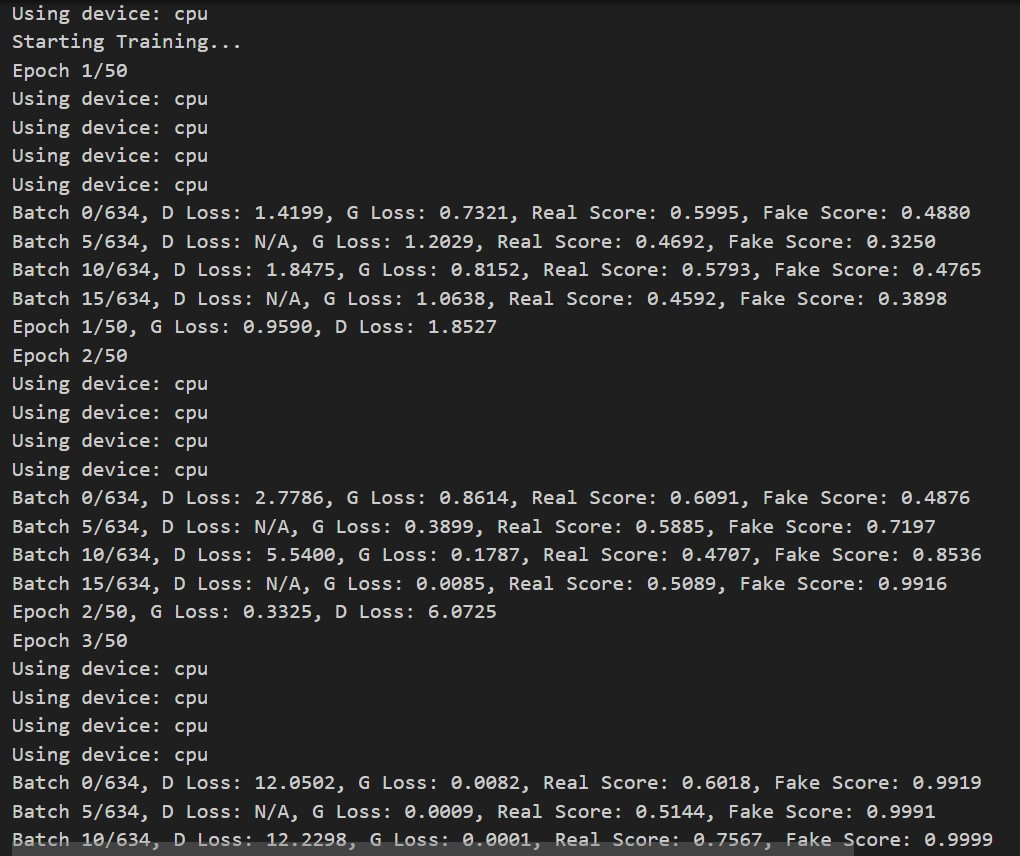
\includegraphics[width=0.85\textwidth]{tracking_progress.jpg}
    \caption{Epoch-wise training progress showing generator and discriminator loss curves.}
    \label{fig:training-progress}
\end{figure}

\end{document}
